\section{Caso de estudio y datos}
\label{sec:caso-datos}

%-------------------------------------------
\subsection{Emplazamiento y geometría de la fundación}
\label{sec:emplazamiento-geometria}
%-------------------------------------------

El caso de estudio corresponde a una fundación de hormigón masivo para un aerogenerador, evaluada bajo las condiciones meteorológicas del sector de Los Ángeles, región del Biobío. El sitio de referencia es el Parque Eólico El Rosal y el punto de consulta climática se fija en la latitud $-37{,}277929^{\circ}$ y la longitud $-72{,}368271^{\circ}$. Estas coordenadas representan el punto meteorológico del caso docente y no la ubicación exacta de una fundación construida. De esta manera, el estudio combina una geometría común del proyecto académico con condiciones ambientales asociadas al sitio asignado.

La geometría se obtiene del archivo oficial de trabajo \texttt{fundacion.ifc}, conservado en el repositorio. El modelo contiene cinco objetos de clase \texttt{IfcFooting}, denominados \texttt{Vertida\_01} a \texttt{Vertida\_05}, que conforman un cuerpo de base octogonal, una transición de sección decreciente y un pedestal superior cilíndrico, como se muestra en la Figura~\ref{fig:geometria-ifc}. La extensión máxima en planta es de $18\times18\,\mathrm{m}$ y la altura total alcanza $4{,}30\,\mathrm{m}$. El pedestal ocupa el tramo entre las cotas $3{,}30$ y $4{,}30\,\mathrm{m}$, con un diámetro nominal de $7\,\mathrm{m}$.

\begin{figure}[htbp]
  \centering
  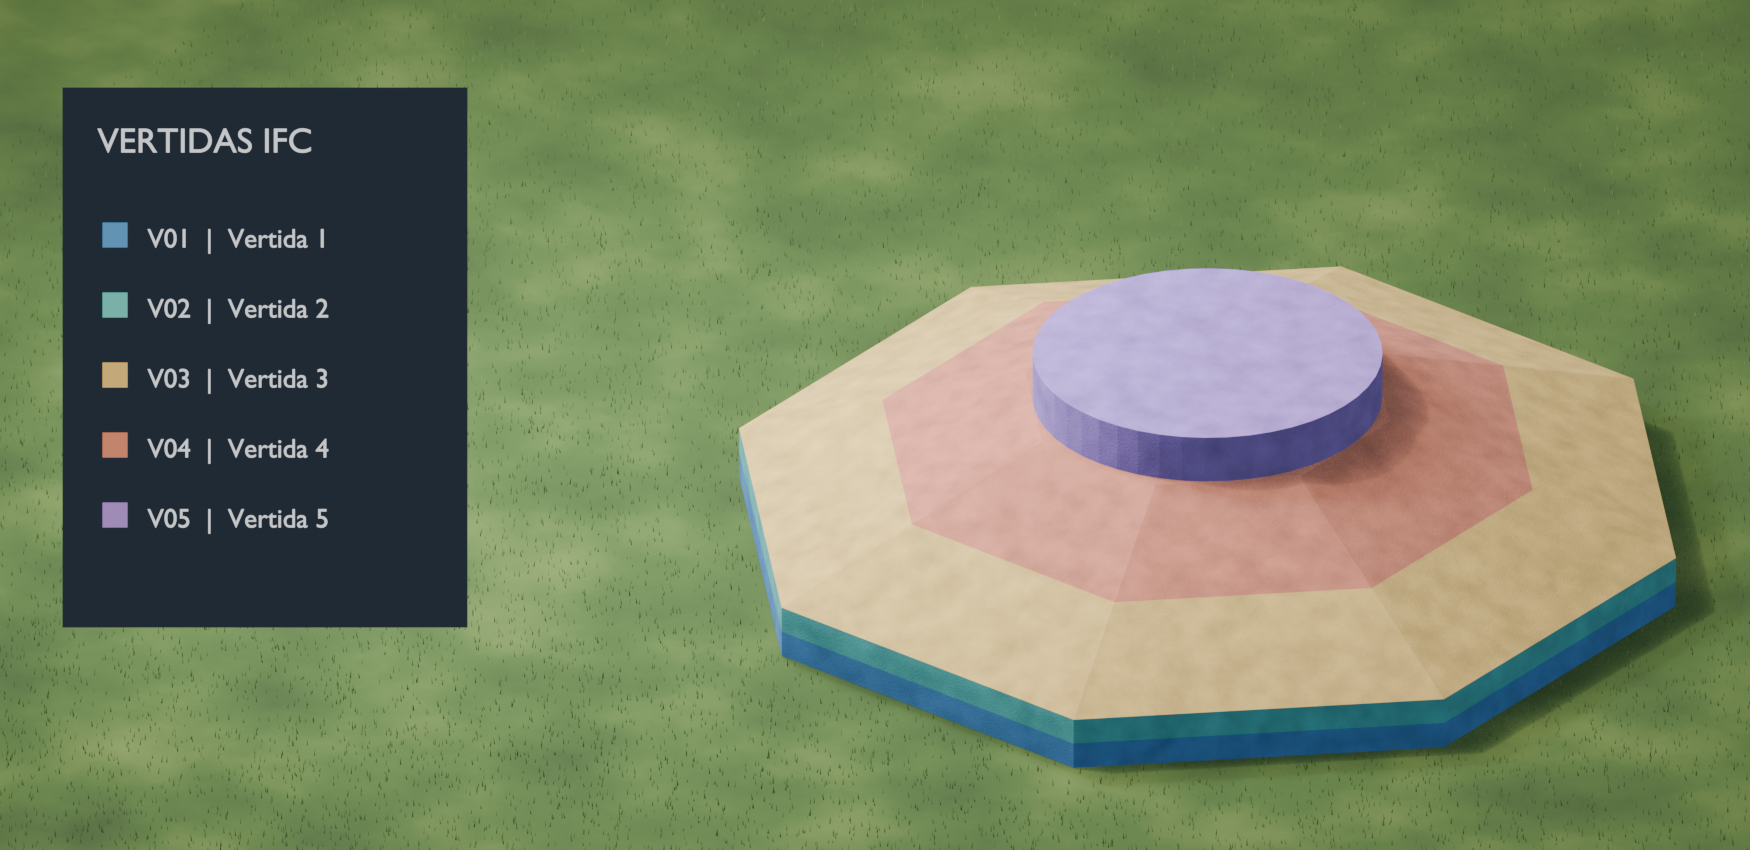
\includegraphics[width=0.85\linewidth]{Imagenes/geometria_ifc.png}
  \caption{Geometría de la fundación y vertidas definidas en el modelo IFC}
  \label{fig:geometria-ifc}
  \captionsetup{skip=2pt}
  \caption*{Fuente: elaboración propia en Blender/Bonsai a partir de \texttt{fundacion.ifc}.}
\end{figure}

La Tabla~\ref{tab:geometria-ifc} resume las cotas, las dimensiones envolventes y los volúmenes obtenidos de las superficies trianguladas del IFC. La suma de los volúmenes de las cinco vertidas es de $636{,}775\,\mathrm{m^3}$. Las dimensiones envolventes indican la extensión máxima de cada pieza; su producto no representa el volumen del sólido, debido a la forma octogonal y a las superficies inclinadas. Esta distinción evita sustituir la geometría real del modelo por bloques rectangulares de mayor volumen.

\begin{table}[htbp]
  \centering
  \caption{Características geométricas de los objetos de la fundación}
  \label{tab:geometria-ifc}
  \small
  \begin{tabular}{lccc}
    \toprule
    Objeto & Intervalo de cota [m] & Envolvente $x\times y\times z$ [m] & Volumen [$\mathrm{m^3}$] \\
    \midrule
    \texttt{Vertida\_01} & $0{,}00$--$0{,}55$ & $18{,}00\times18{,}00\times0{,}55$ & $147{,}626$ \\
    \texttt{Vertida\_02} & $0{,}55$--$1{,}10$ & $18{,}00\times18{,}00\times0{,}55$ & $147{,}626$ \\
    \texttt{Vertida\_03} & $1{,}10$--$2{,}20$ & $18{,}00\times18{,}00\times1{,}10$ & $214{,}224$ \\
    \texttt{Vertida\_04} & $2{,}20$--$3{,}30$ & $12{,}50\times12{,}50\times1{,}10$ & $88{,}925$ \\
    \texttt{Vertida\_05} & $3{,}30$--$4{,}30$ & $7{,}00\times7{,}00\times1{,}00$ & $38{,}375$ \\
    \midrule
    Conjunto & $0{,}00$--$4{,}30$ & $18{,}00\times18{,}00\times4{,}30$ & $636{,}775$ \\
    \bottomrule
  \end{tabular}
  \captionsetup{skip=2pt}
  \caption*{Fuente: extracción propia del archivo IFC.}
\end{table}

Se distinguen la base en contacto con el terreno, las superficies laterales y la coronación expuestas al ambiente. La representación térmica considera el volumen de hormigón, sin resolver explícitamente las armaduras ni los anclajes del aerogenerador.

La partición geométrica del IFC se mantiene como referencia de identidad y forma, pero se distingue de la secuencia constructiva evaluada. Aunque los objetos conservan el nombre de vertidas, la propuesta distribuye la colocación en once capas físicas sin alterar la geometría final. La definición de esas capas, su cronología y los controles térmicos se presentan en los apartados siguientes. Asimismo, la comparación entre el volumen geométrico y el volumen representado por la malla se desarrolla al describir la voxelización.


%-------------------------------------------
%-------------------------------------------
\subsection{Representación BIM y voxelización}
\label{sec:BIM-Voxelización}
%-------------------------------------------

El flujo de trabajo parte del modelo BIM almacenado en formato IFC y transforma su geometría en una malla cartesiana para el cálculo térmico. La lectura se realiza con IfcOpenShell, que permite obtener los vértices y las caras trianguladas de los sólidos \citep{ifcopenshellGeometria}. Se aplican las posiciones de los objetos y la conversión de unidades a metros, conservando las coordenadas locales del proyecto. Los nombres y los identificadores de los objetos se mantienen para vincular la representación numérica con el archivo de origen.

La información geométrica utilizada comprende las superficies trianguladas, las dimensiones y la posición relativa de las cinco piezas. El lector también recupera sus propiedades constructivas, pero el cálculo del plan adoptado utiliza un cronograma externo de once capas, junto con las temperaturas de colocación y los controles definidos para la comparación. Por tanto, los valores iniciales almacenados en los campos del IFC no se adoptan automáticamente como condiciones del estudio. Las propiedades térmicas del material y los datos ambientales se incorporan desde archivos de configuración independientes.

La voxelización consiste en dividir la caja envolvente del conjunto en celdas cúbicas de lado $h$. El origen de la malla coincide con el mínimo geométrico del IFC, aproximadamente $(-9,-9,0)\,\mathrm{m}$, y se mantiene al refinar. Cada centro de celda se clasifica respecto de las superficies trianguladas: la celda se considera ocupada si el centro está dentro de alguno de los sólidos o sobre su frontera, con una tolerancia geométrica de $10^{-7}\,\mathrm{m}$. La pertenencia a varios objetos no duplica su ocupación. 

Este criterio asigna el volumen completo de la celda y no calcula fracciones de intersección, por lo que aproxima las superficies curvas e inclinadas mediante un contorno escalonado. Para cuantificar esta aproximación se calcula el volumen discretizado como:
\begin{equation}
    V_h=N_h \cdot h^3
\end{equation}
tal que $N_h$ es el número de celdas ocupadas y $h$ es el lado de cada celda. Este volumen se compara con la referencia geométrica $V_{\mathrm{IFC}}=636{,}775\,\mathrm{m^3}$, obtenida como la suma de los volúmenes de las piezas trianguladas.
La diferencia firmada es: 
\begin{equation}
    \Delta V=V_h-V_{\mathrm{IFC}}
\end{equation}
y su magnitud relativa es:
\begin{equation}
    \varepsilon_V=\frac{|\Delta V|}{V_{\mathrm{IFC}}} \cdot 100
\end{equation}
tal que $\varepsilon_V$ es la magnitud de la diferencia relativa expresada en porcentaje. La Tabla~\ref{tab:volumen-voxelizacion} presenta los valores recuperados de las geometrías guardadas para las dos resoluciones utilizadas. Las diferencias se calculan con los valores sin redondear; el redondeo se aplica únicamente para su presentación.

\begin{table}[htbp]
  \centering
  \caption{Comparación del volumen geométrico y discretizado de la fundación}
  \label{tab:volumen-voxelizacion}
  \small
  \begin{tabular}{ccccc}
    \toprule
    $h$ [m] & $N_h$ & $V_h$ [$\mathrm{m^3}$] & $\Delta V$ [$\mathrm{m^3}$] & $\varepsilon_V$ [\%] \\
    \midrule
    $0{,}40$ & $10\,011$ & $640{,}704$ & $+3{,}929$ & $0{,}617$ \\
    $0{,}20$ & $79\,868$ & $638{,}944$ & $+2{,}169$ & $0{,}341$ \\
    \bottomrule
  \end{tabular}
  \captionsetup{skip=2pt}
  \caption*{Fuente: elaboración propia a partir de las geometrías archivadas.}
\end{table}

En ambas mallas el volumen discretizado supera al geométrico, aunque la diferencia disminuye al pasar de $0{,}40$ a $0{,}20\,\mathrm{m}$. Este resultado caracteriza la aproximación global del volumen, pero no demuestra por sí solo la exactitud de las superficies ni la convergencia de las temperaturas. Para calcular la duración de colocación se conserva el volumen físico del plan, sin sustituirlo por el volumen voxelizado; así, un cambio de malla no modifica artificialmente el objetivo constructivo.

Finalmente, las celdas ocupadas se agrupan por altura en las once capas del plan, manteniendo esa misma partición física en ambas resoluciones. La máscara geométrica representa la fundación completa y se distingue del dominio activo: durante el cálculo solo participan las capas cuya colocación ya se ha activado. La activación y la identificación de las caras exteriores permiten actualizar las superficies de intercambio a medida que avanza la construcción. Su formulación térmica se desarrolla en las secciones de modelo continuo y discretización.

%-------------------------------------------
%-------------------------------------------
\subsection{Parámetros térmicos y condiciones de colocación}
\label{sec:Parametros y condiciones}
%-------------------------------------------

Para comparar los planes en las mismas condiciones, se conservan los datos del material, del ambiente y de los sistemas de protección y refrigeración; entre las dos alternativas cambia la tasa de colocación. Las Tablas~\ref{tab:param-materiales} a~\ref{tab:param-plan} reúnen estos parámetros y señalan su procedencia. La clasificación bibliográfico corresponde a valores publicados; ajustado, a resultados obtenidos al ajustar un modelo a datos; y supuesto, a valores o decisiones adoptados para el estudio. Un dato se presenta como medido únicamente si se dispone de antecedentes que acrediten su medición.

La densidad y el calor específico se toman del archivo docente de hidratación \citep{fuentesDocentes}. La conductividad del hormigón, en cambio, se adopta como un valor fijo que no se ajustó a mediciones de la fundación. Ese archivo también entrega las curvas que describen cuánto calor genera el hormigón a medida que envejece; su origen y tratamiento se explican en el apartado siguiente.

Para la madera y las mantas se utilizan los valores publicados para AraucoPly y Aislanglass \citep{araucoCatalogo,volcanCES}. La referencia de AraucoPly corresponde al catálogo internacional de esa familia de tableros, por lo que su aplicación al producto utilizado en obra requiere comprobar que sus características sean equivalentes. En ambos materiales, la información publicada permite representar su resistencia térmica, pero no sustituye la comprobación del montaje de las protecciones.

\begin{table}[htbp]
  \centering
  \caption{Propiedades del hormigón y de las protecciones térmicas}
  \label{tab:param-materiales}
  \small
  \setlength{\tabcolsep}{4pt}
  \begin{tabular}{p{1.4cm}p{4.0cm}p{2.1cm}p{2.0cm}p{3.8cm}p{2.7cm}}
    \toprule
    Símbolo & Significado & Unidad & Valor & Procedencia & Clasificación \\
    \midrule
    $\rho$ & Densidad del hormigón & $\mathrm{kg\,m^{-3}}$ & $2\,476$ & Archivo docente & Supuesto adoptado \\
    $c_p$ & Calor específico & $\mathrm{J\,kg^{-1}\,K^{-1}}$ & $1\,023$ & Archivo docente & Supuesto adoptado \\
    $k_c$ & Conductividad del hormigón & $\mathrm{W\,m^{-1}\,K^{-1}}$ & $2$ & Configuración térmica & Supuesto \\
    $\dot q_{h,m}(a)$ & Fuente por edad y curva & $\mathrm{W\,m^{-3}}$ & $8$ funciones tabuladas & Archivo docente & Ajustado \\
    $e_m$ & Espesor de madera & $\mathrm{m}$ & $0{,}018$ & Referencia AraucoPly & Bibliográfico \\
    $k_m$ & Conductividad de madera & $\mathrm{W\,m^{-1}\,K^{-1}}$ & $0{,}158$ & AraucoPly, tabla $11$ & Bibliográfico \\
    $e_a$ & Espesor de cada manta & $\mathrm{m}$ & $0{,}040$ & Ficha Aislanglass & Bibliográfico \\
    $k_a$ & Conductividad de cada manta & $\mathrm{W\,m^{-1}\,K^{-1}}$ & $0{,}042$ & Ficha Aislanglass & Bibliográfico \\
    \bottomrule
  \end{tabular}
  \captionsetup{skip=2pt}
  \caption*{Fuente: Archivo docente de hidratación, documentación de ARAUCO y Volcán, y configuración del estudio.}
\end{table}

Para representar la pérdida de calor hacia el suelo, se supone que el terreno mantiene una temperatura constante y que el calor atraviesa una distancia equivalente de suelo. No se calcula cómo se calienta o enfría el terreno con el tiempo. El intercambio con el aire depende del viento y se estima con la relación de McAdams presentada en la documentación de EnergyPlus \citep{energyplusMcAdams}, expresada en unidades SI como:
\begin{equation}
    h_c(t)=5{,}7+3{,}8~v_2(t)
\end{equation}
tal que $v_2(t)$ es la velocidad horaria del viento en $\mathrm{m\,s^{-1}}$, referida a una altura de $2\,\mathrm{m}$, y $h_c(t)$ relaciona el intercambio de calor con la diferencia de temperatura entre la superficie y el aire. 
\newpage
La altura de referencia y el exponente usado para ajustar el viento se adoptan como supuestos. También se fijan la fracción de radiación solar absorbida por la superficie, denominada absortancia; su capacidad de emitir radiación térmica, representada por la emisividad; y la fracción de radiación solar reflejada por el entorno, o albedo. Estos valores no proceden de mediciones del acabado de la fundación. La Tabla~\ref{tab:param-ambiente} los reúne junto con los parámetros del suelo y de la sombra. El subíndice de $h_c$ permite distinguir este coeficiente del lado de celda $h$.

\begin{table}[htbp]
  \centering
  \caption{Parámetros del suelo y del intercambio con el ambiente}
  \label{tab:param-ambiente}
  \small
  \setlength{\tabcolsep}{4pt}
  \begin{tabular}{p{1.4cm}p{3.5cm}p{2.1cm}p{1.8cm}p{3.8cm}p{2.2cm}}
    \toprule
    Símbolo & Significado & Unidad & Valor & Procedencia & Clasificación \\
    \midrule
    $T_g$ & Temperatura del reservorio de suelo & $^{\circ}\mathrm{C}$ & $15$ & Configuración del suelo & Supuesto \\
    $L_g$ & Longitud equivalente de suelo & $\mathrm{m}$ & $0{,}50$ & Configuración del suelo & Supuesto \\
    $k_g$ & Conductividad equivalente del suelo & $\mathrm{W\,m^{-1}\,K^{-1}}$ & $1{,}2$ & Configuración del suelo & Supuesto \\
    $h_c(t)$ & Coeficiente convectivo & $\mathrm{W\,m^{-2}\,K^{-1}}$ & Variable & McAdams, según EnergyPlus & Bibliográfico \\
    $z_v$ & Altura representativa del viento & $\mathrm{m}$ & $2$ & Configuración ambiental & Supuesto \\
    $\gamma_v$ & Exponente del perfil de viento & Adimensional & $0{,}14$ & Configuración ambiental & Supuesto \\
    $\alpha_{\mathrm{SW}}$ & Absortancia solar exterior & Adimensional & $0{,}60$ & Configuración radiativa & Supuesto \\
    $\varepsilon$ & Emisividad de onda larga & Adimensional & $0{,}90$ & Configuración radiativa & Supuesto \\
    $r_g$ & Albedo del entorno & Adimensional & $0{,}20$ & Configuración radiativa & Supuesto \\
    $\tau_{\mathrm{SW}}$ & Transmitancia solar de la sombra & Adimensional & $0{,}10$ & Protección idealizada & Supuesto \\
    \bottomrule
  \end{tabular}
  \captionsetup{skip=2pt}
  \caption*{Fuente: Documentación de EnergyPlus y configuración del estudio.}
\end{table}
Los planes parten del $19$ de noviembre de $2026$ a las $10{:}00$, con desfase UTC$-03{:}00$. La propuesta considera dos frentes de hasta $30\,\mathrm{m^3/h}$ cada uno, sin esperas entre las once capas y con hormigón colocado a $12\,^{\circ}\mathrm{C}$. Los laterales se cubren con madera y dos mantas, mientras que la cara superior recibe las dos mantas sin madera. El retiro se cuenta desde la colocación de cada capa: la madera permanece $72\,\mathrm{h}$, la primera manta $240\,\mathrm{h}$ y la segunda $504\,\mathrm{h}$. Al retirar la última manta se incorpora una sombra idealizada que deja pasar el $10~\%$ de la radiación solar y se conserva hasta el final del seguimiento de $672\,\mathrm{h}$, manteniendo las demás condiciones de intercambio. Las edades de retiro forman parte de la programación simulada. Los resultados respaldan el cumplimiento de los criterios térmicos al mantener la última manta hasta las $504\,\mathrm{h}$ de edad de cada capa y aplicar posteriormente la sombra, bajo los escenarios y supuestos evaluados. No se buscó determinar la menor edad de retiro admisible. Su aplicación en obra requiere comprobar las temperaturas y la resistencia del hormigón.
\newpage

El efecto de los circuitos se incorpora como una extracción de calor distribuida en la zona refrigerable, con agua a temperatura uniforme y una potencia total limitada. Un circuito solo puede abrirse después de quedar cubierto por hormigón y cuando todos sus puntos de control alcanzan al menos $19\,^{\circ}\mathrm{C}$; se cierra si alguno baja a $18\,^{\circ}\mathrm{C}$ o menos. La diferencia entre ambas temperaturas evita aperturas y cierres repetidos alrededor de un único umbral. Este control puede actuar durante todo el seguimiento, sin una fecha fija de apagado general. El coeficiente $U_v$ representa el intercambio térmico equivalente adoptado: no se obtiene del caudal nominal de los ramales. El modelo no calcula el paso de calor a través de la pared del tubo y su contacto con el hormigón, ni el calentamiento del agua a lo largo del recorrido. Por ello, el comportamiento calculado todavía requiere una comprobación del diseño hidráulico y de la transferencia real de calor.

\begin{table}[htbp]
  \centering
  \caption{Condiciones de colocación y refrigeración adoptadas}
  \label{tab:param-plan}
  \small
  \setlength{\tabcolsep}{4pt}
  \begin{tabular}{p{1.4cm}p{3.8cm}p{2.1cm}p{2.0cm}p{3.7cm}p{2.8cm}}
    \toprule
    Símbolo & Significado & Unidad & Valor o conjunto & Procedencia & Clasificación \\
    \midrule
    $q$ & Tasa de colocación comparada & $\mathrm{m^3\,h^{-1}}$ & $55$ y $60$ & Familia de planes & Supuesto de capacidad \\
    $T_{\mathrm{col}}$ & Temperatura de colocación & $^{\circ}\mathrm{C}$ & $12$ & Configuración del plan & Supuesto \\
    $n_L$ & Número de capas físicas & Adimensional & $11$ & Partición adoptada & Supuesto de diseño \\
    $e_L$ & Espesor nominal de capa; última capa & $\mathrm{m}$ & $0{,}40$; $0{,}30$ & Partición adoptada & Supuesto de diseño \\
    $a_r$ & Edades de retiro: madera y mantas & $\mathrm{h}$ & $72$; $240$; $504$ & Protección evaluada & Supuesto de diseño \\
    $n_r$ & Número de circuitos & Adimensional & $9$ & Anteproyecto del equipo & Supuesto de diseño \\
    $T_w$ & Temperatura uniforme del agua & $^{\circ}\mathrm{C}$ & $18$ & Refrigeración equivalente & Supuesto \\
    $U_v$ & Coeficiente volumétrico de extracción & $\mathrm{W\,m^{-3}\,K^{-1}}$ & $5$ & Refrigeración equivalente & Supuesto \\
    $P_{\max}$ & Potencia máxima global & $\mathrm{kW}$ & $15$ & Refrigeración equivalente & Supuesto \\
    $V_r$ & Volumen refrigerable & $\mathrm{m^3}$ & $414{,}016$ & Máscara del anteproyecto & Supuesto de diseño \\
    $Q_r$ & Caudal nominal por ramal abierto & $\mathrm{L\,min^{-1}}$ & $18$ & Anteproyecto del equipo & Supuesto de diseño \\
    $Q_{\mathrm{tot}}$ & Caudal total con bypass & $\mathrm{L\,min^{-1}}$ & $162$ & Anteproyecto del equipo & Supuesto de diseño \\
    $T_{\mathrm{on}}$, $T_{\mathrm{off}}$ & Umbrales de apertura y cierre & $^{\circ}\mathrm{C}$ & $19$; $18$ & Control por histéresis & Supuesto de diseño \\
    \bottomrule
  \end{tabular}
  \captionsetup{skip=2pt}
  \caption*{Fuente: Configuración final del estudio y anteproyecto de circuitos del equipo.}
\end{table}


%-------------------------------------------
\subsection{Datos de hidratación y tratamiento de las ocho curvas}
\label{sec:Hidratación y curvas}
%-------------------------------------------

Para describir el calor de hidratación se utilizan las ocho curvas del archivo docente \texttt{source\_terms.txt}: \texttt{M1\_SS} a \texttt{M4\_SS} y \texttt{M1\_22A} a \texttt{M4\_22A}. Cada curva indica la potencia térmica generada por unidad de volumen de hormigón, en $\mathrm{W\,m^{-3}}$. Estos valores se estimaron a partir de registros de temperatura de probetas, ajustando un modelo para determinar la generación de calor que explica las temperaturas observadas \citep{fuentesDocentes}. Este procedimiento se denomina inversión. Las curvas entregadas ya son fuentes de calor, por lo que se incorporan sin volver a derivar una temperatura adiabática.
\newpage

El archivo describe probetas cilíndricas de radio $0{,}0375\,\mathrm{m}$ y altura $0{,}15\,\mathrm{m}$. Para estimar el calor generado se utilizó un modelo de volúmenes finitos que aprovecha la simetría del cilindro y considera sus pérdidas hacia el ambiente mediante una conductancia de borde fija de $2{,}5\,\mathrm{W\,m^{-2}\,K^{-1}}$. La curva se representó con B-splines cúbicos, es decir, funciones polinómicas unidas de forma suave, con $16$ funciones base. El ajuste incorporó regularización de Tikhonov, con una penalización de segundas diferencias de $0{,}05$, y correcciones de los desplazamientos de lectura de cada sensor. Estos procedimientos buscan controlar las oscilaciones del ajuste y las diferencias sistemáticas entre sensores. Se conservó ese procesamiento docente, sin repetirlo para el estudio de la fundación.

Las etiquetas \texttt{M1} a \texttt{M4} identifican las probetas. Las curvas \texttt{SS} corresponden a registros del $13$ al $20$ de abril de $2025$, y las \texttt{22A}, al $22$ de abril del mismo año. En ambos grupos se toma como edad cero el comienzo de la parte del registro que se conservó, situada dos horas después del inicio original. Ese instante se usa como aproximación del inicio de hidratación de cada capa. El calor de las dos horas descartadas no se reconstruye, lo que limita la representación de las primeras edades.

No se dispone de antecedentes suficientes para confirmar que las ocho curvas provengan de ensayos independientes de una misma dosificación. Se conservan como ocho respuestas posibles del material dentro del modelo, sin atribuirles una representatividad estadística que los datos no demuestran. Además, el archivo señala que las curvas \texttt{22A} tienen menor confianza, porque el sensor ambiental no explica adecuadamente la respuesta de las probetas a los cambios diarios de temperatura. El error de ajuste reportado, medido como raíz del error cuadrático medio, es de aproximadamente $0{,}4\,\mathrm{K}$ para \texttt{22A} y de $0{,}1$--$0{,}2\,\mathrm{K}$ para \texttt{SS}. Se mantienen las ocho curvas en la comparación, reconociendo que la calidad del ajuste difiere entre ambas campañas.

Se conserva cada serie hasta su última muestra disponible. Los valores \texttt{NaN} que aparecen después indican que el registro terminó; no se interpretan como mediciones de calor nulo. No se encontraron datos faltantes dentro de los tramos conservados ni se aplicó un nuevo suavizado. Las muestras están separadas por $600\,\mathrm{s}$, equivalentes a diez minutos, y se utiliza ese intervalo para evitar diferencias debidas al redondeo de las horas en el archivo. El calor acumulado se obtiene sumando el aporte entre muestras mediante la regla del trapecio:
\begin{equation}
    H_{m,j}=\sum_{r=0}^{j-1}
    \frac{\dot q_{m,r}+\dot q_{m,r+1}}{2}
    (a_{r+1}-a_r), \qquad H_{m,0}=0,
\end{equation}
tal que $m$ identifica la curva, $j$ y $r$ indican las posiciones de las muestras y $a_r$ es la edad en segundos. El valor $H_{m,j}$ representa el calor generado hasta esa edad por unidad de volumen de hormigón, en $\mathrm{J\,m^{-3}}$.

Para incorporar estos datos al cálculo, se unen con segmentos rectos los valores del calor acumulado $H_m(a)$. Así se puede obtener la energía generada entre dos edades, aunque no coincidan con las muestras originales. La pendiente de cada segmento representa la fuente efectiva utilizada en ese intervalo:
\begin{equation}
    \dot q_{h,m}(a)=\frac{H_{m,j+1}-H_{m,j}}{a_{j+1}-a_j},
    \qquad a_j\leq a<a_{j+1}.
\end{equation}
\newpage

Durante un paso que va de la edad $a_i$ a la edad $a_f$, el calor incorporado por unidad de volumen es:
\begin{equation}
    H_m(a_f)-H_m(a_i)
\end{equation}
De esta forma, el aporte depende del calor acumulado entre ambos instantes y se conserva aunque el paso de cálculo difiera del intervalo de los datos. La Figura~\ref{fig:hidratacion-fuentes} muestra las ocho curvas entregadas, las fuentes utilizadas durante las primeras $48\,\mathrm{h}$ y sus calores acumulados.

La Tabla~\ref{tab:hidratacion-calor} resume el máximo de cada curva y su calor total. Al integrar las fuentes se recuperan, a la precisión de los archivos, los acumulados guardados en los ocho CSV. El mismo resultado se obtiene al sumar los aportes con intervalos de $300\,\mathrm{s}$. Esta comprobación confirma que el tratamiento conserva la energía de los datos; no permite concluir que el ajuste de las probetas o las temperaturas de la fundación hayan sido validados con mediciones independientes.

Después de la última muestra se mantiene constante el calor acumulado. Esto equivale a suponer que no se genera más calor después de aproximadamente $240{,}333\,\mathrm{h}$ para \texttt{SS} y $163\,\mathrm{h}$ para \texttt{22A}. Se trata de una hipótesis para completar el período sin datos, y no de una observación del fin de la hidratación. De hecho, la última muestra de \texttt{M1\_SS} todavía indica una fuente de $1{,}57\,\mathrm{W\,m^{-3}}$.

En cada simulación se asigna una misma curva completa a todas las capas, pero la edad comienza a contarse al activar cada una. Esto supone que el material de toda la fundación comparte una misma respuesta de hidratación. La generación de calor depende únicamente de esa edad, sin modificar su velocidad según la temperatura calculada. Cada curva se conserva por separado: no se combinan partes de distintas series ni se utiliza una curva promedio para reemplazarlas. Los pesos asignados y sus consecuencias se explican en la sección de incertidumbre.

\begin{table}[htbp]
  \centering
  \caption{Duración de registro, máximos tabulados y calor acumulado de las fuentes de hidratación}
  \label{tab:hidratacion-calor}
  \small
  \begin{tabular}{lccc}
    \toprule
    Curva & Edad final [h] & Máximo tabulado [$\mathrm{W\,m^{-3}}$] & Calor [$\mathrm{MJ\,m^{-3}}$] \\
    \midrule
    \texttt{M1\_SS}  & $240{,}333$ & $467{,}75$ & $88{,}148$ \\
    \texttt{M2\_SS}  & $240{,}333$ & $531{,}11$ & $95{,}715$ \\
    \texttt{M3\_SS}  & $240{,}333$ & $553{,}01$ & $94{,}149$ \\
    \texttt{M4\_SS}  & $240{,}333$ & $568{,}94$ & $100{,}166$ \\
    \texttt{M1\_22A} & $163{,}000$ & $473{,}38$ & $61{,}212$ \\
    \texttt{M2\_22A} & $163{,}000$ & $625{,}29$ & $82{,}446$ \\
    \texttt{M3\_22A} & $163{,}000$ & $589{,}70$ & $73{,}289$ \\
    \texttt{M4\_22A} & $163{,}000$ & $596{,}08$ & $73{,}628$ \\
    \bottomrule
  \end{tabular}
  \captionsetup{skip=2pt}
  \caption*{Fuente: Elaboración propia a partir del archivo docente y de los acumulados conservados en el repositorio.}
\end{table}
\newpage

\begin{figure}[htbp]
  \centering
  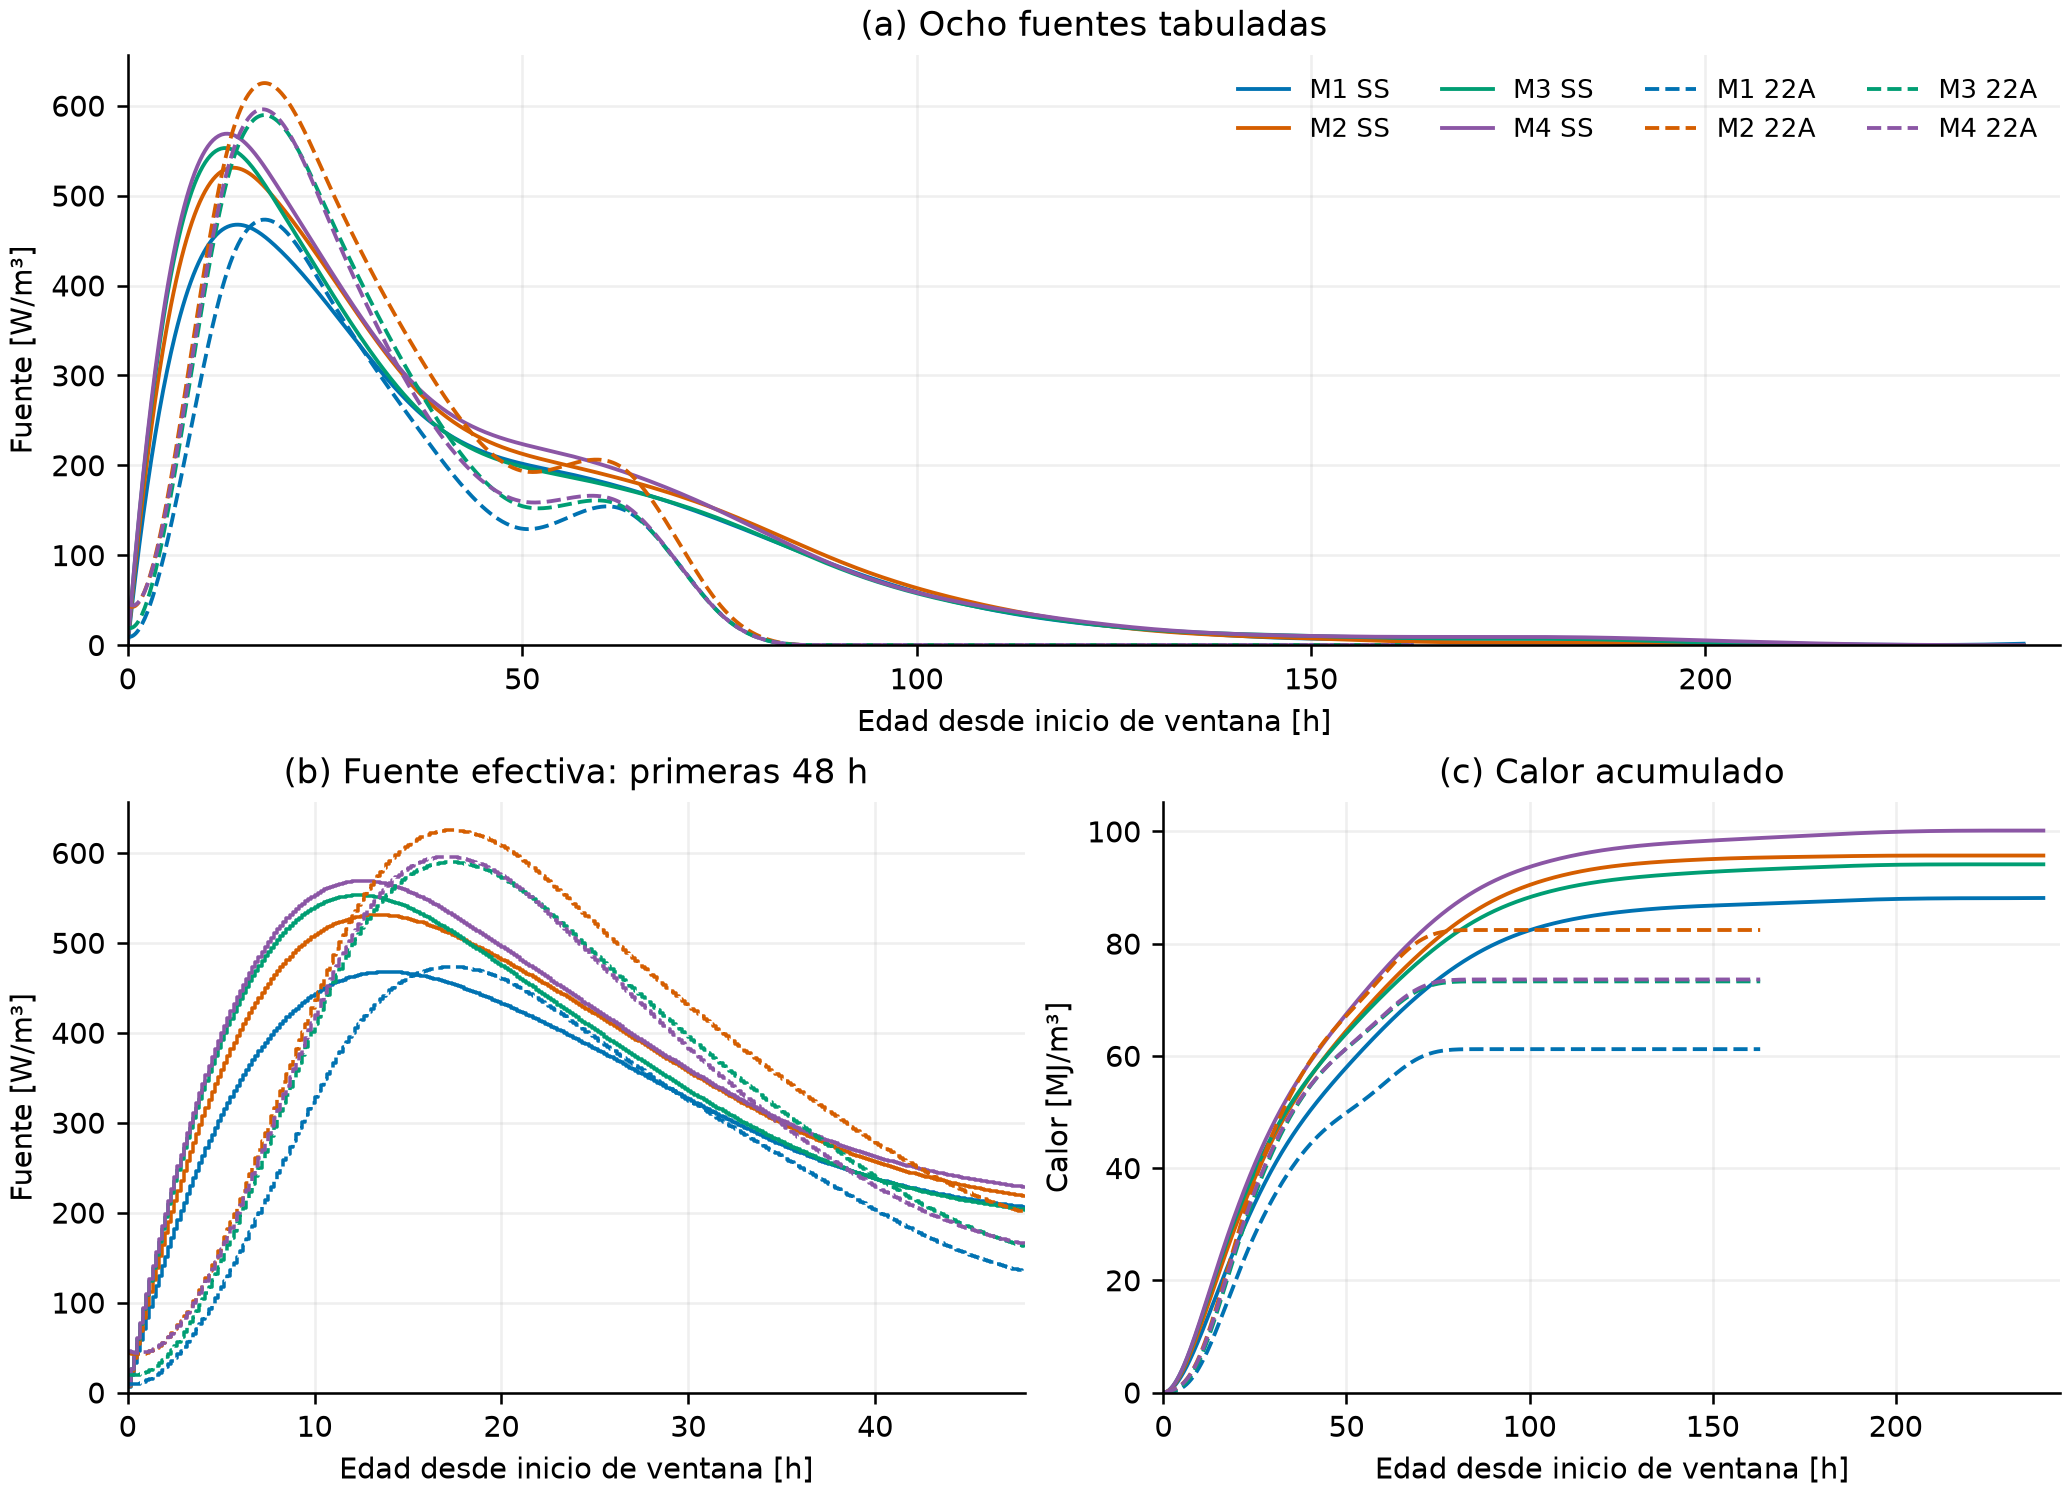
\includegraphics[width=0.98\linewidth]{Imagenes/hidratacion_fuentes_calor.png}
  \caption{Fuentes tabuladas, fuente efectiva y calor acumulado de las ocho curvas de hidratación}
  \label{fig:hidratacion-fuentes}
  \captionsetup{skip=2pt}
  \caption*{Fuente: Elaboración propia a partir de \texttt{source\_terms.txt} y de los archivos tabulares del modelo.}
\end{figure}


%-------------------------------------------
\subsection{Datos meteorológicos y tratamiento temporal}
\label{sec:Meteorologicos}
%-------------------------------------------

El clima se representa mediante tres historias horarias de los años $2023$, $2024$ y $2025$, obtenidas de ERA5 a través de la API histórica de Open-Meteo \citep{openmeteoHistorico}. ERA5 es un reanálisis: combina observaciones y un modelo atmosférico para reconstruir las condiciones del pasado. Por ello, estas series se utilizan como escenarios históricos del sitio y no como pronósticos del tiempo que ocurriría durante la construcción en $2026$.

Las consultas utilizan las coordenadas del apartado~\ref{sec:emplazamiento-geometria}. La respuesta del proveedor corresponde al punto de grilla de latitud $-37{,}25^{\circ}$ y longitud $-72{,}25^{\circ}$. Esta diferencia refleja la representación espacial del producto; los valores no son mediciones tomadas en la posición exacta de la fundación. Las solicitudes conservadas permiten identificar tanto las coordenadas pedidas como las devueltas.
\newpage

Cada archivo abarca del $19$ de noviembre al $17$ de diciembre de su año, desde las $00{:}00$ del primer día hasta las $23{:}00$ del último, en UTC, con $696$ marcas horarias. Los datos iniciales incluyen temperatura del aire, viento y radiación global. Posteriormente se descargaron archivos complementarios para incorporar las variables necesarias para radiación, sin reemplazar los anteriores. La Tabla~\ref{tab:descargas-clima} identifica ambas descargas; los instantes se muestran hasta el segundo, y los metadatos conservan su precisión original.

\begin{table}[htbp]
  \centering
  \caption{Descargas de las historias meteorológicas utilizadas}
  \label{tab:descargas-clima}
  \small
  \begin{tabular}{lcc}
    \toprule
    Historia & Descarga inicial [UTC] & Descarga complementaria [UTC] \\
    \midrule
    ERA5-$2023$ & $17/11/2026$, $01{:}37{:}07$ & $18/11/2026$, $20{:}02{:}51$ \\
    ERA5-$2024$ & $17/11/2026$, $01{:}37{:}06$ & $18/11/2026$, $20{:}02{:}53$ \\
    ERA5-$2025$ & $17/11/2026$, $01{:}37{:}07$ & $18/11/2026$, $20{:}02{:}54$ \\
    \bottomrule
  \end{tabular}
  \captionsetup{skip=2pt}
  \caption*{Fuente: metadatos de los archivos descargados de Open-Meteo.}
\end{table}

Para relacionar cada historia con la obra, se toma el $19$ de noviembre de su año a las $10{:}00$, UTC$-03{:}00$, como inicio de tiempo relativo. Esa hora corresponde a las $13{:}00$ UTC. A partir de ella se conserva la secuencia horaria completa y se aplica al inicio constructivo del $19$ de noviembre de $2026$, declarado en el apartado anterior. Así se mantienen los ciclos diarios y la relación entre las variables de cada historia. La posición solar se calcula con las fechas históricas correspondientes. Los archivos se almacenan en UTC y el inicio de obra se identifica con la zona \texttt{America/Santiago}, evitando confundir ambas referencias.

La Tabla~\ref{tab:variables-clima} resume las variables que intervienen en los intercambios térmicos. La temperatura del aire, el viento y la radiación global de las descargas complementarias coinciden exactamente con los archivos iniciales en las tres historias. La radiación directa horizontal también se conserva para comprobar su suma con la difusa frente a la global. La temperatura del cielo se estima a partir del punto de rocío y la nubosidad total; no se dispone de una medición infrarroja del cielo. El suelo mantiene el tratamiento equivalente descrito en el apartado~\ref{sec:Parametros y condiciones}, sin utilizar una serie de temperatura del terreno.

\begin{table}[htbp]
  \centering
  \caption{Variables meteorológicas y uso en el modelo térmico}
  \label{tab:variables-clima}
  \small
  \setlength{\tabcolsep}{4pt}
  \begin{tabular}{p{5.0cm}p{1.8cm}p{9.0cm}}
    \toprule
    Variable & Unidad & Uso \\
    \midrule
    Temperatura del aire a $2\,\mathrm{m}$ & $^{\circ}\mathrm{C}$ & Intercambio convectivo y cálculo del entorno radiativo \\
    Velocidad del viento a $10\,\mathrm{m}$ & $\mathrm{m\,s^{-1}}$ & Ajuste a $2\,\mathrm{m}$ y cálculo del coeficiente convectivo \\
    Radiación global horizontal (GHI) & $\mathrm{W\,m^{-2}}$ & Radiación sobre caras superiores y reflexión del entorno \\
    Radiación directa normal (DNI) & $\mathrm{W\,m^{-2}}$ & Componente directa según la orientación de cada cara \\
    Radiación difusa horizontal (DHI) & $\mathrm{W\,m^{-2}}$ & Componente difusa sobre las caras expuestas \\
    Punto de rocío a $2\,\mathrm{m}$ & $^{\circ}\mathrm{C}$ & Estimación de la emisión térmica del cielo \\
    Nubosidad total & $\%$ & Aproximación de la nubosidad opaca en la estimación del cielo \\
    \bottomrule
  \end{tabular}
  \captionsetup{skip=2pt}
  \caption*{Fuente: Archivos meteorológicos y tratamiento implementado en el modelo.}
\end{table}
\newpage

Entre las marcas horarias se interpola linealmente la temperatura del aire, el punto de rocío y la nubosidad. El coeficiente convectivo se mantiene constante durante cada hora, calculado con el viento de su marca inicial. Las irradiancias representan el promedio de la hora precedente \citep{openmeteoHistorico}: para el intervalo entre dos marcas se utiliza el dato de la marca final, con la posición solar evaluada en el punto medio. Este tratamiento respeta el intervalo temporal al que pertenece la energía solar.

Las Figuras~\ref{fig:clima-ambiente} y~\ref{fig:clima-radiacion} muestran las series utilizadas durante las $672\,\mathrm{h}$ y el coeficiente convectivo calculado. La línea vertical en $336\,\mathrm{h}$ distingue el horizonte obligatorio del seguimiento extendido. Se verificó la continuidad horaria y la ausencia de valores faltantes en las variables utilizadas. La cobertura disponible permite completar ambos horizontes sin repetir días, rellenar huecos ni prolongar la última temperatura. Las diferencias entre estas tres historias representan parte de la variación climática posible; su número limitado no permite tratarlas como una descripción completa de los extremos meteorológicos del sitio.

\begin{figure}[htbp]
  \centering
  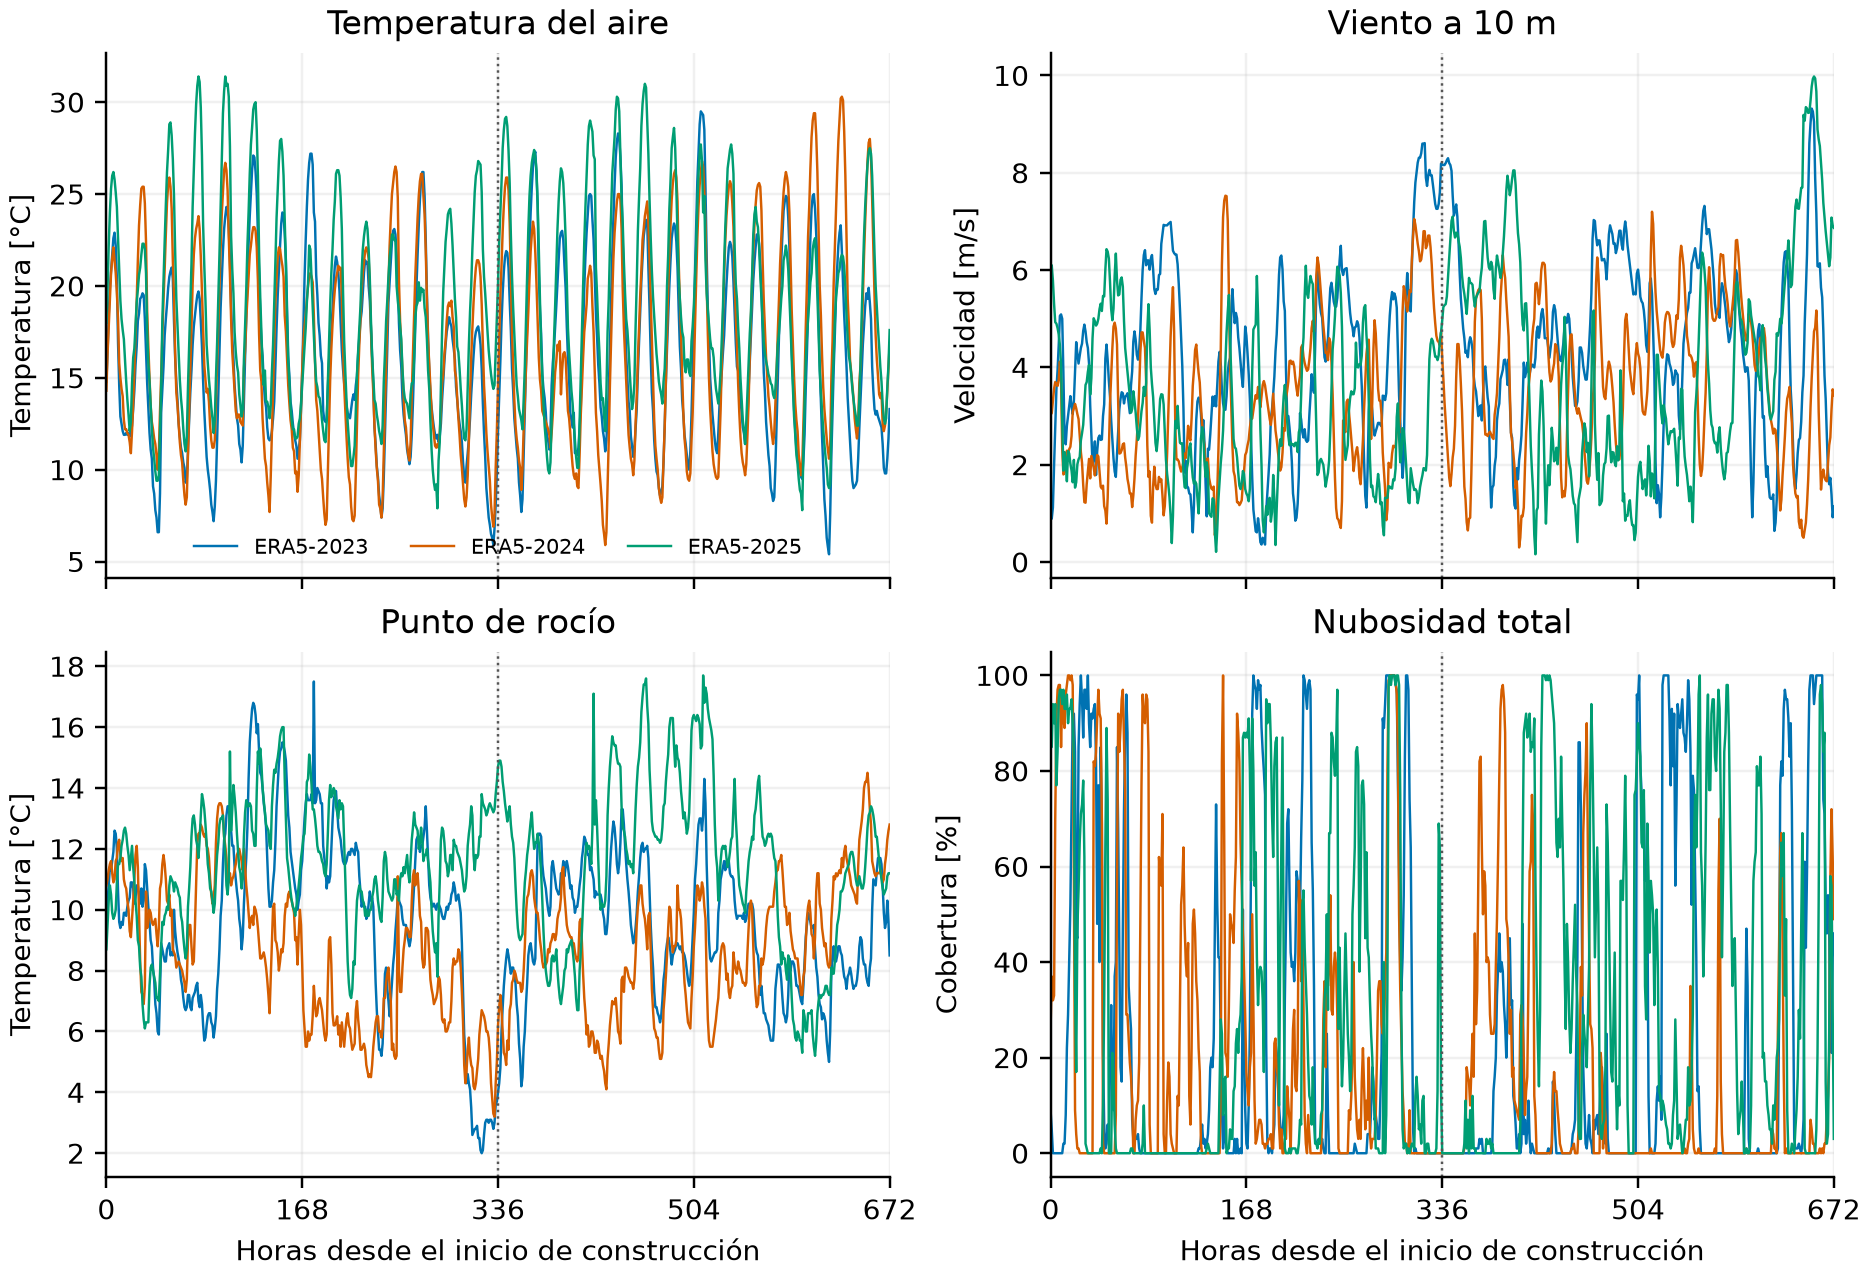
\includegraphics[width=0.95\linewidth]{Imagenes/clima_ambiente.png}
  \caption{Temperatura del aire, viento, punto de rocío y nubosidad de las tres historias climáticas}
  \label{fig:clima-ambiente}
  \captionsetup{skip=2pt}
  \caption*{Fuente: Elaboración propia a partir de los archivos ERA5 descargados de Open-Meteo.}
\end{figure}
\newpage
\begin{figure}[h]
  \centering
  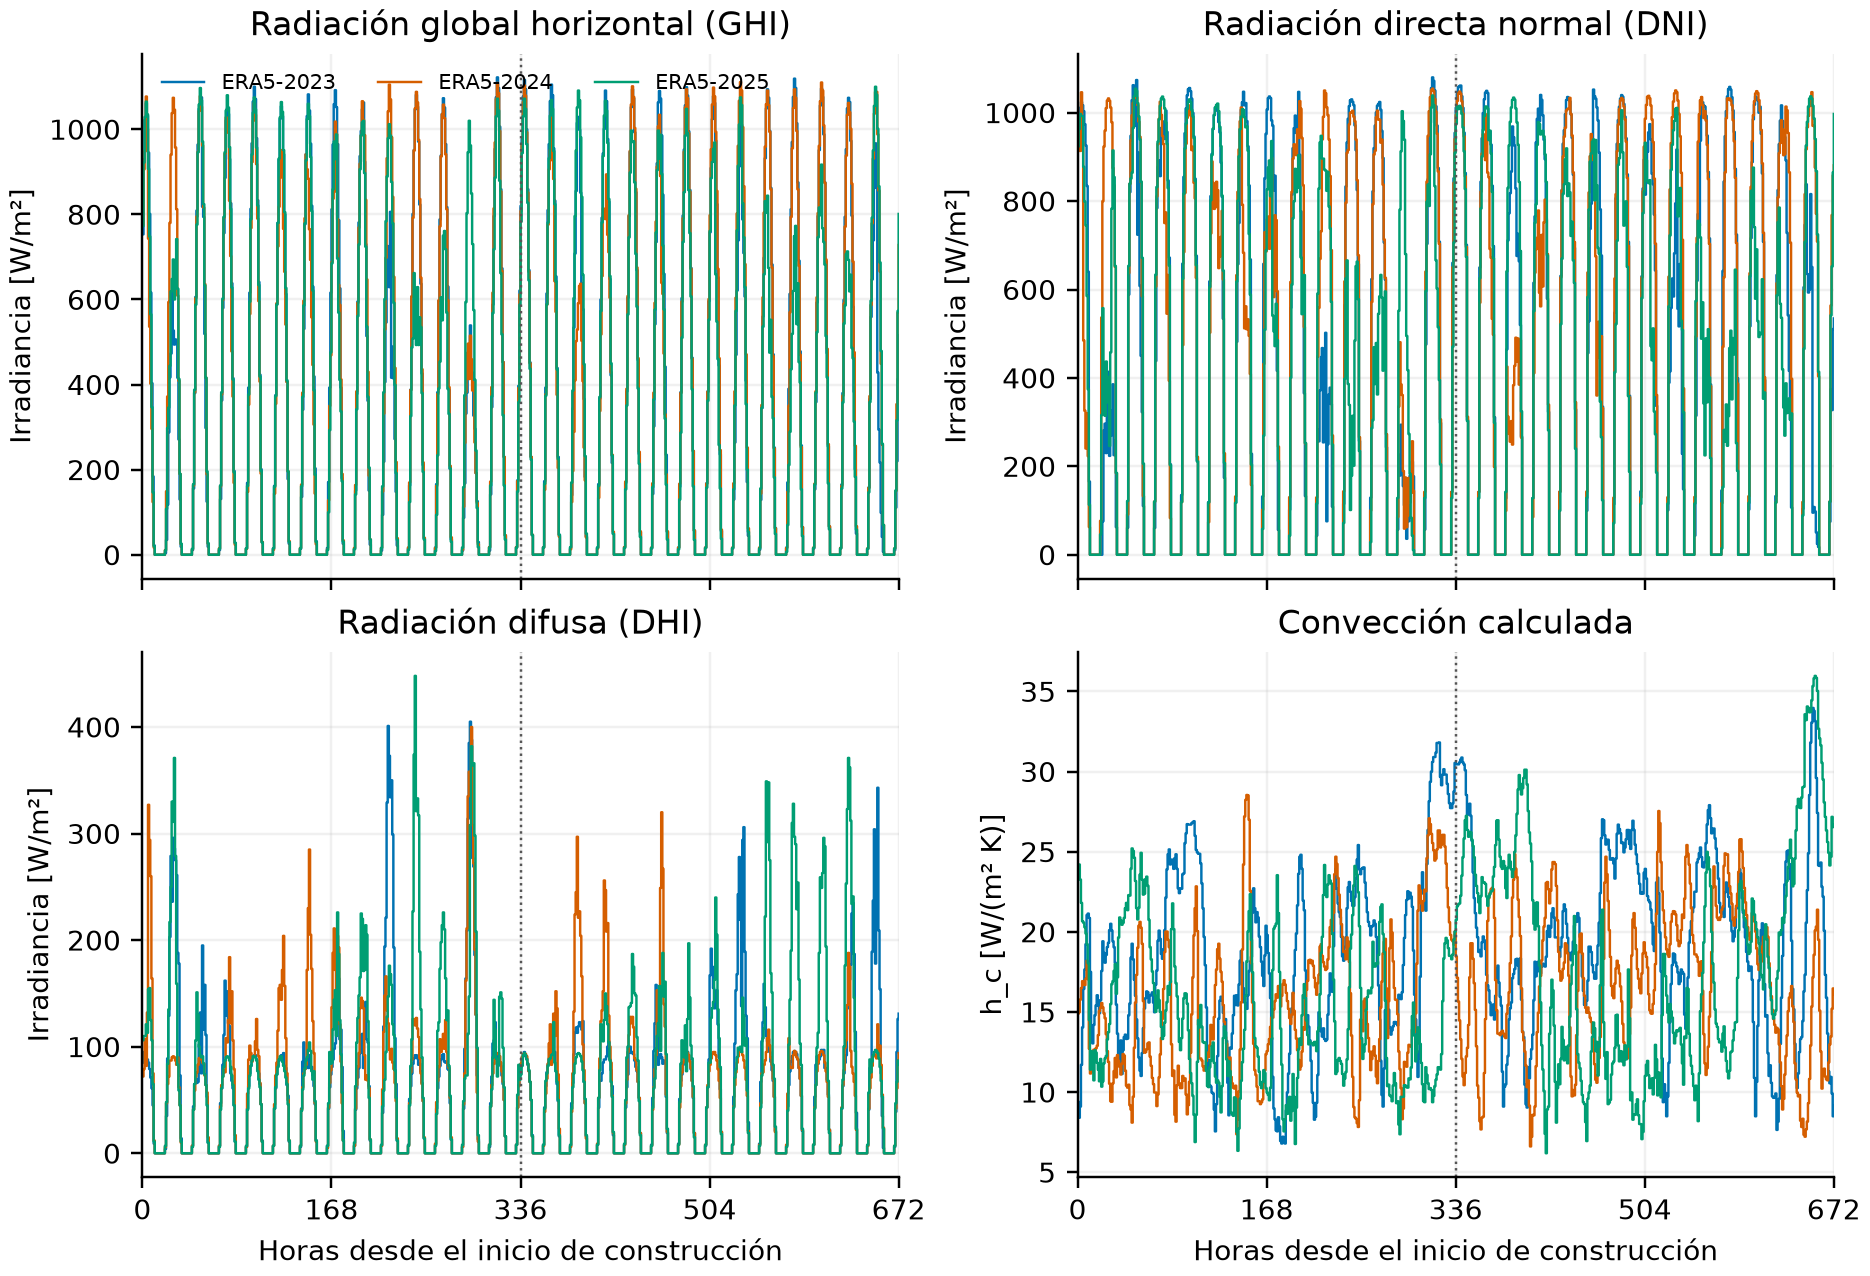
\includegraphics[width=0.95\linewidth]{Imagenes/clima_radiacion_conveccion.png}
  \caption{Radiación solar y coeficiente convectivo utilizados en las tres historias climáticas}
  \label{fig:clima-radiacion}
  \captionsetup{skip=2pt}
  \caption*{Fuente: Elaboración propia a partir de los archivos ERA5 y de la correlación convectiva adoptada.}
\end{figure}

En ambas figuras, el eje horizontal representa las horas transcurridas desde el inicio de construcción y los colores distinguen las tres historias climáticas. Los ejes verticales indican la variable representada y su unidad.

La Figura~\ref{fig:clima-ambiente} muestra los ciclos diarios de temperatura y las diferencias de viento, punto de rocío y nubosidad entre las historias. En la Figura~\ref{fig:clima-radiacion} se observa la alternancia de la radiación solar entre el día y la noche, mientras que el coeficiente convectivo cambia con la velocidad del viento. Estas variaciones hacen que las condiciones de intercambio de calor entre la fundación y el ambiente cambien durante el seguimiento.

%-------------------------------------------
\subsection{Trazabilidad y congelación de los datos}
\label{sec:Trazabilidad}
%-------------------------------------------

La comparación utiliza copias locales de los datos, conservadas sin cambios durante la campaña de cálculo. Cada archivo meteorológico guarda la respuesta original del proveedor y los metadatos de la consulta: dirección de acceso, variables, coordenadas, unidades, zona horaria y fecha de descarga. El manifiesto de radiación vincula cada archivo complementario con su descarga inicial y registra la coincidencia de las variables comunes. Esto permite reconstruir qué información se utilizó sin depender de una nueva consulta al servicio.

\newpage
El repositorio conserva las descargas históricas en \path{datos/clima/reanalisis}, las complementarias en \path{datos/clima/radiacion} y los pronósticos previos en \path{datos/clima/forecasts}. Entre estos últimos existen archivos descargados el $10$ y el $17$ de noviembre de $2026$. Se mantienen como antecedentes de las etapas anteriores; la comparación final de este artículo se basa en las tres historias ERA5 descritas, sin mezclarlas con esos pronósticos. La ampliación de variables del $18$ de noviembre corresponde a una descarga efectivamente registrada, no a una reconstrucción retrospectiva de información supuestamente disponible antes.

La configuración final identifica el IFC, las curvas de hidratación, los planes y las condiciones térmicas. Los resultados por escenario registran esas referencias junto con huellas SHA-256, códigos que permiten comprobar si un archivo ha cambiado. Se contrastaron las referencias climáticas de las $72$ corridas archivadas del cierre: las dos tasas de colocación y la confirmación fina de la propuesta utilizan los mismos datos meteorológicos para cada historia. De esta forma, la comparación no obtiene ventajas por cambiar el clima entre planes o resoluciones.

Para facilitar la revisión del artículo, se archivaron las series mostradas en las figuras, los metadatos y las huellas de los insumos en \path{entregas/F01/articulo/datos}. Las configuraciones y métricas completas permanecen en sus carpetas de origen. Cualquier corrección posterior a la defensa debe conservar la versión previa y registrar qué cambió, por qué y si modifica la recomendación. Los identificadores de los commits de defensa y de entrega final se documentarán junto con los comandos de reproducción en el anexo correspondiente; las huellas de archivos no sustituyen esos identificadores.
